% mnras_template.tex 
%
% LaTeX template for creating an MNRAS paper
%
% v3.0 released 14 May 2015
% (version numbers match those of mnras.cls)
%
% Copyright (C) Royal Astronomical Society 2015
% Authors:
% Keith T. Smith (Royal Astronomical Society)

% Change log
%
% v3.0 May 2015
%    Renamed to match the new package name
%    Version number matches mnras.cls
%    A few minor tweaks to wording
% v1.0 September 2013
%    Beta testing only - never publicly released
%    First version: a simple (ish) template for creating an MNRAS paper

%%%%%%%%%%%%%%%%%%%%%%%%%%%%%%%%%%%%%%%%%%%%%%%%%%
% Basic setup. Most papers should leave these options alone.
\documentclass[fleqn,usenatbib]{mnras}

% MNRAS is set in Times font. If you don't have this installed (most LaTeX
% installations will be fine) or prefer the old Computer Modern fonts, comment
% out the following line
\usepackage{newtxtext,newtxmath}
% Depending on your LaTeX fonts installation, you might get better results with one of these:
%\usepackage{mathptmx}
%\usepackage{txfonts}

% Use vector fonts, so it zooms properly in on-screen viewing software
% Don't change these lines unless you know what you are doing
\usepackage[T1]{fontenc}
\usepackage{ae,aecompl}


%%%%% AUTHORS - PLACE YOUR OWN PACKAGES HERE %%%%%

% Only include extra packages if you really need them. Common packages are:
\usepackage{graphicx}	% Including figure files
\usepackage{amsmath}	% Advanced maths commands
\usepackage{amssymb}	% Extra maths symbols

%%%%%%%%%%%%%%%%%%%%%%%%%%%%%%%%%%%%%%%%%%%%%%%%%%

%%%%% AUTHORS - PLACE YOUR OWN COMMANDS HERE %%%%%

% Please keep new commands to a minimum, and use \newcommand not \def to avoid
% overwriting existing commands. Example:
%\newcommand{\pcm}{\,cm$^{-2}$}	% per cm-squared

%%%%%%%%%%%%%%%%%%%%%%%%%%%%%%%%%%%%%%%%%%%%%%%%%%

%%%%%%%%%%%%%%%%%%% TITLE PAGE %%%%%%%%%%%%%%%%%%%

% Title of the paper, and the short title which is used in the headers.
% Keep the title short and informative.
\title[Short title, max. 45 characters]{The Hercules-Aquila Cloud and Virgo Overdensity with Gaia DR2}

% The list of authors, and the short list which is used in the headers.
% If you need two or more lines of authors, add an extra line using \newauthor
\author[K. T. Smith et al.]{
Keith T. Smith,$^{1}$\thanks{E-mail: mn@ras.org.uk (KTS)}
A. N. Other,$^{2}$
Third Author$^{2,3}$
and Fourth Author$^{3}$
\\
% List of institutions
$^{1}$Royal Astronomical Society, Burlington House, Piccadilly, London W1J 0BQ, UK\\
$^{2}$Department, Institution, Street Address, City Postal Code, Country\\
$^{3}$Another Department, Different Institution, Street Address, City Postal Code, Country
}

% These dates will be filled out by the publisher
\date{Accepted XXX. Received YYY; in original form ZZZ}

% Enter the current year, for the copyright statements etc.
\pubyear{2015}

% Don't change these lines
\begin{document}
\label{firstpage}
\pagerange{\pageref{firstpage}--\pageref{lastpage}}
\maketitle

% Abstract of the paper
\begin{abstract}
200 words for Letters.
No references should appear in the abstract.
\end{abstract}

% Select between one and six entries from the list of approved keywords.
% Don't make up new ones.
\begin{keywords}
keyword1 -- keyword2 -- keyword3
\end{keywords}

%%%%%%%%%%%%%%%%%%%%%%%%%%%%%%%%%%%%%%%%%%%%%%%%%%

%%%%%%%%%%%%%%%%% BODY OF PAPER %%%%%%%%%%%%%%%%%%

\section{Introduction}
Introduction.

\section{Observations}

Normally the next section describes the techniques the authors used.
It is frequently split into subsections, such as Section~\ref{sec:maths} below.

\subsection{Maths}
\label{sec:maths} % used for referring to this section from elsewhere

Simple mathematics can be inserted into the flow of the text e.g. $2\times3=6$
or $v=220$\,km\,s$^{-1}$, but more complicated expressions should be entered
as a numbered equation:

\begin{equation}
    x=\frac{-b\pm\sqrt{b^2-4ac}}{2a}.
	\label{eq:quadratic}
\end{equation}

Refer back to them as e.g. equation~(\ref{eq:quadratic}).

\subsection{Figures and tables}

Figures and tables should be placed at logical positions in the text. Don't
worry about the exact layout, which will be handled by the publishers.

Figures are referred to as e.g. Fig.~\ref{fig:example_figure}.

% Example figure
\begin{figure*}
	% To include a figure from a file named example.*
	% Allowable file formats are eps or ps if compiling using latex
	% or pdf, png, jpg if compiling using pdflatex
	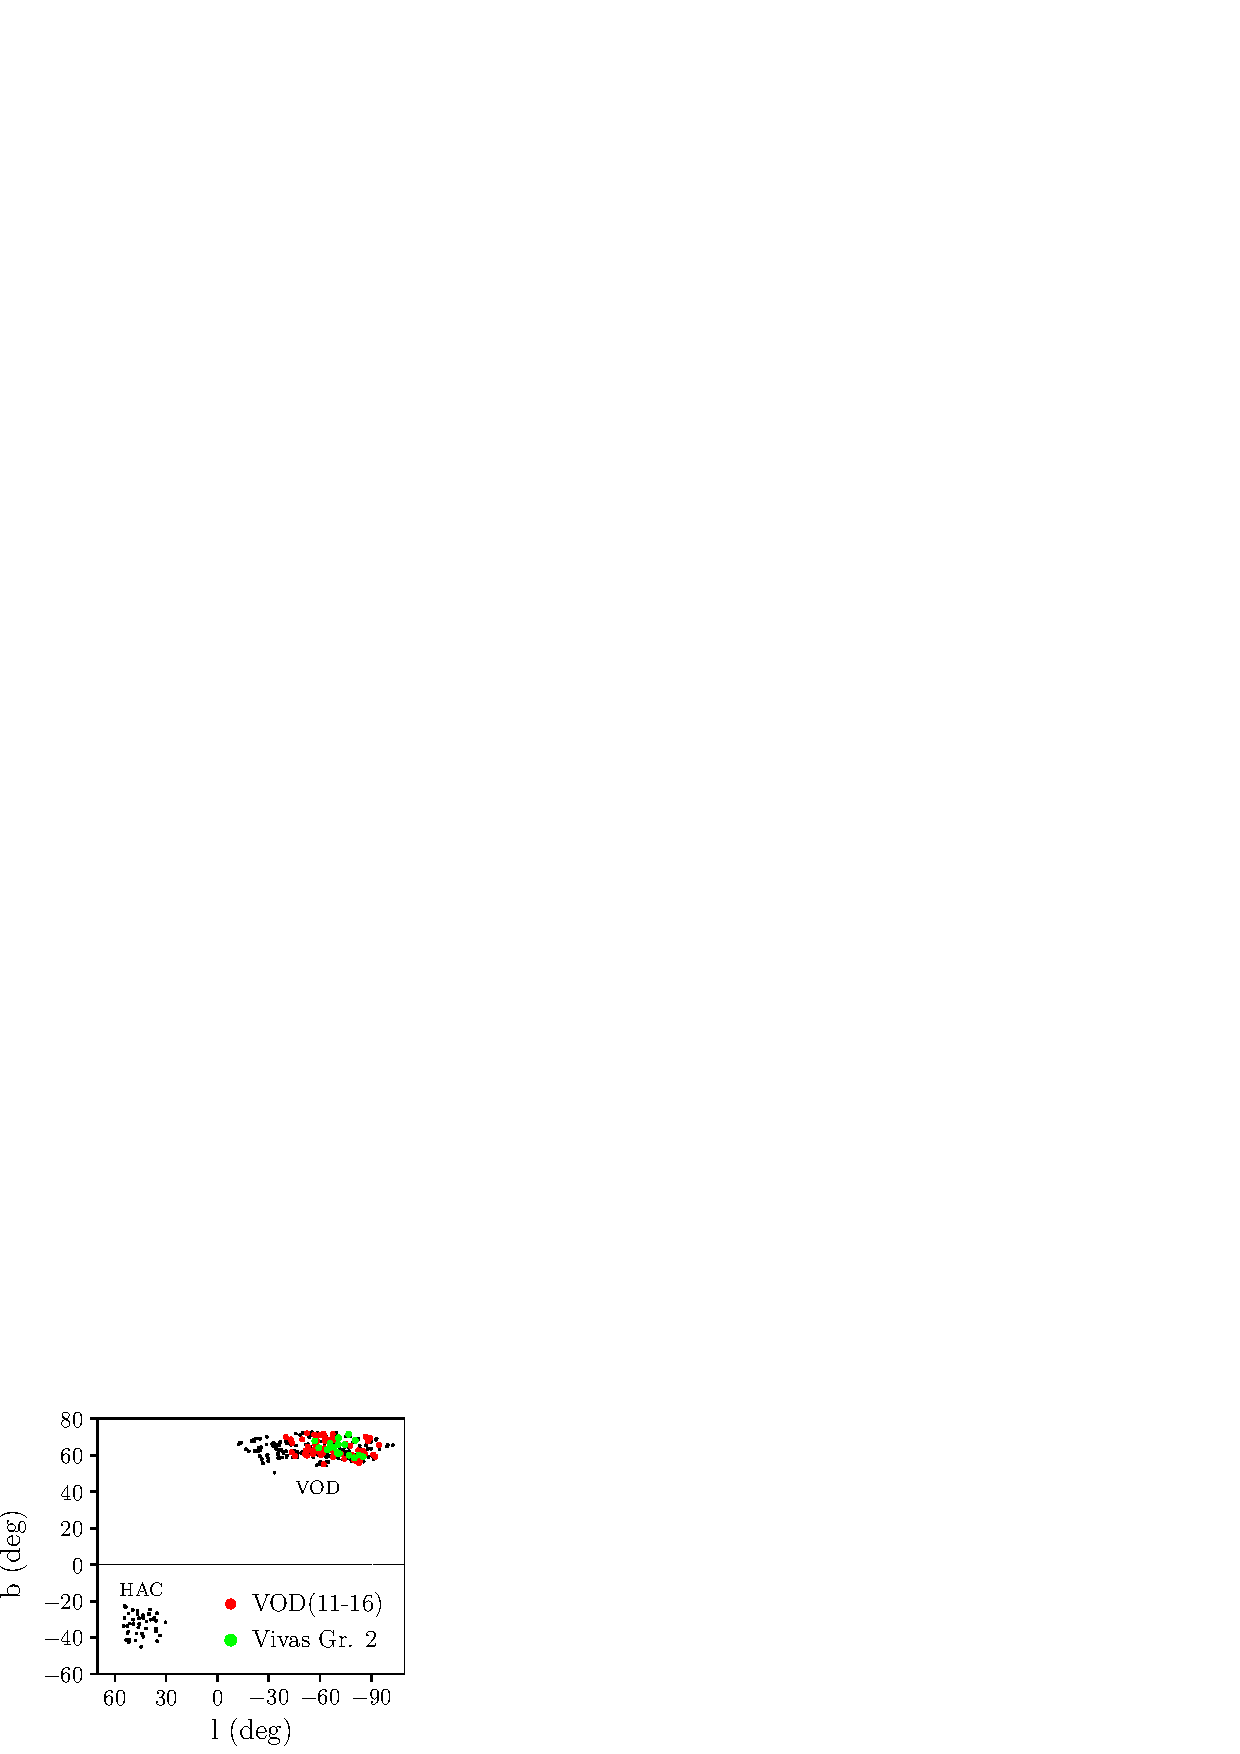
\includegraphics[scale=0.58]{lb.pdf}
	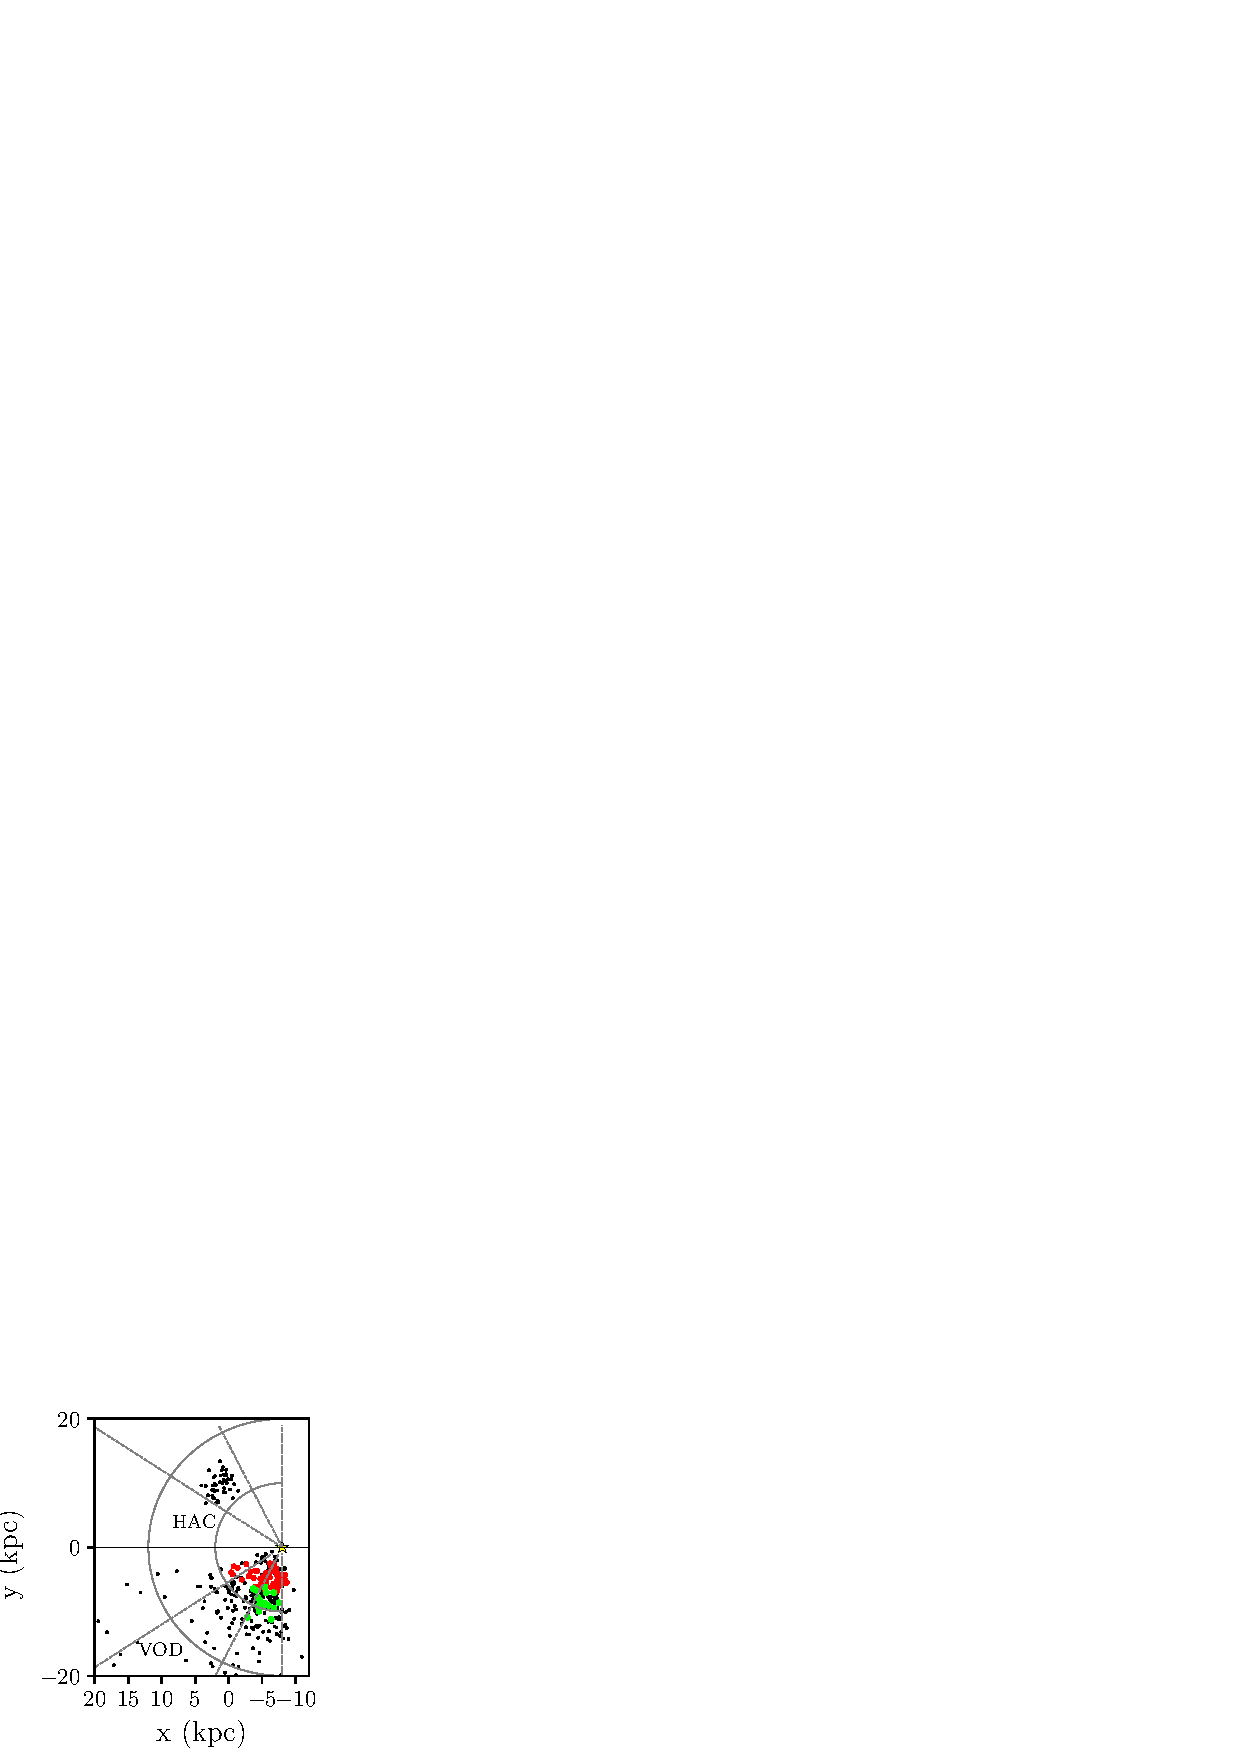
\includegraphics[scale=0.58]{xy.pdf}
	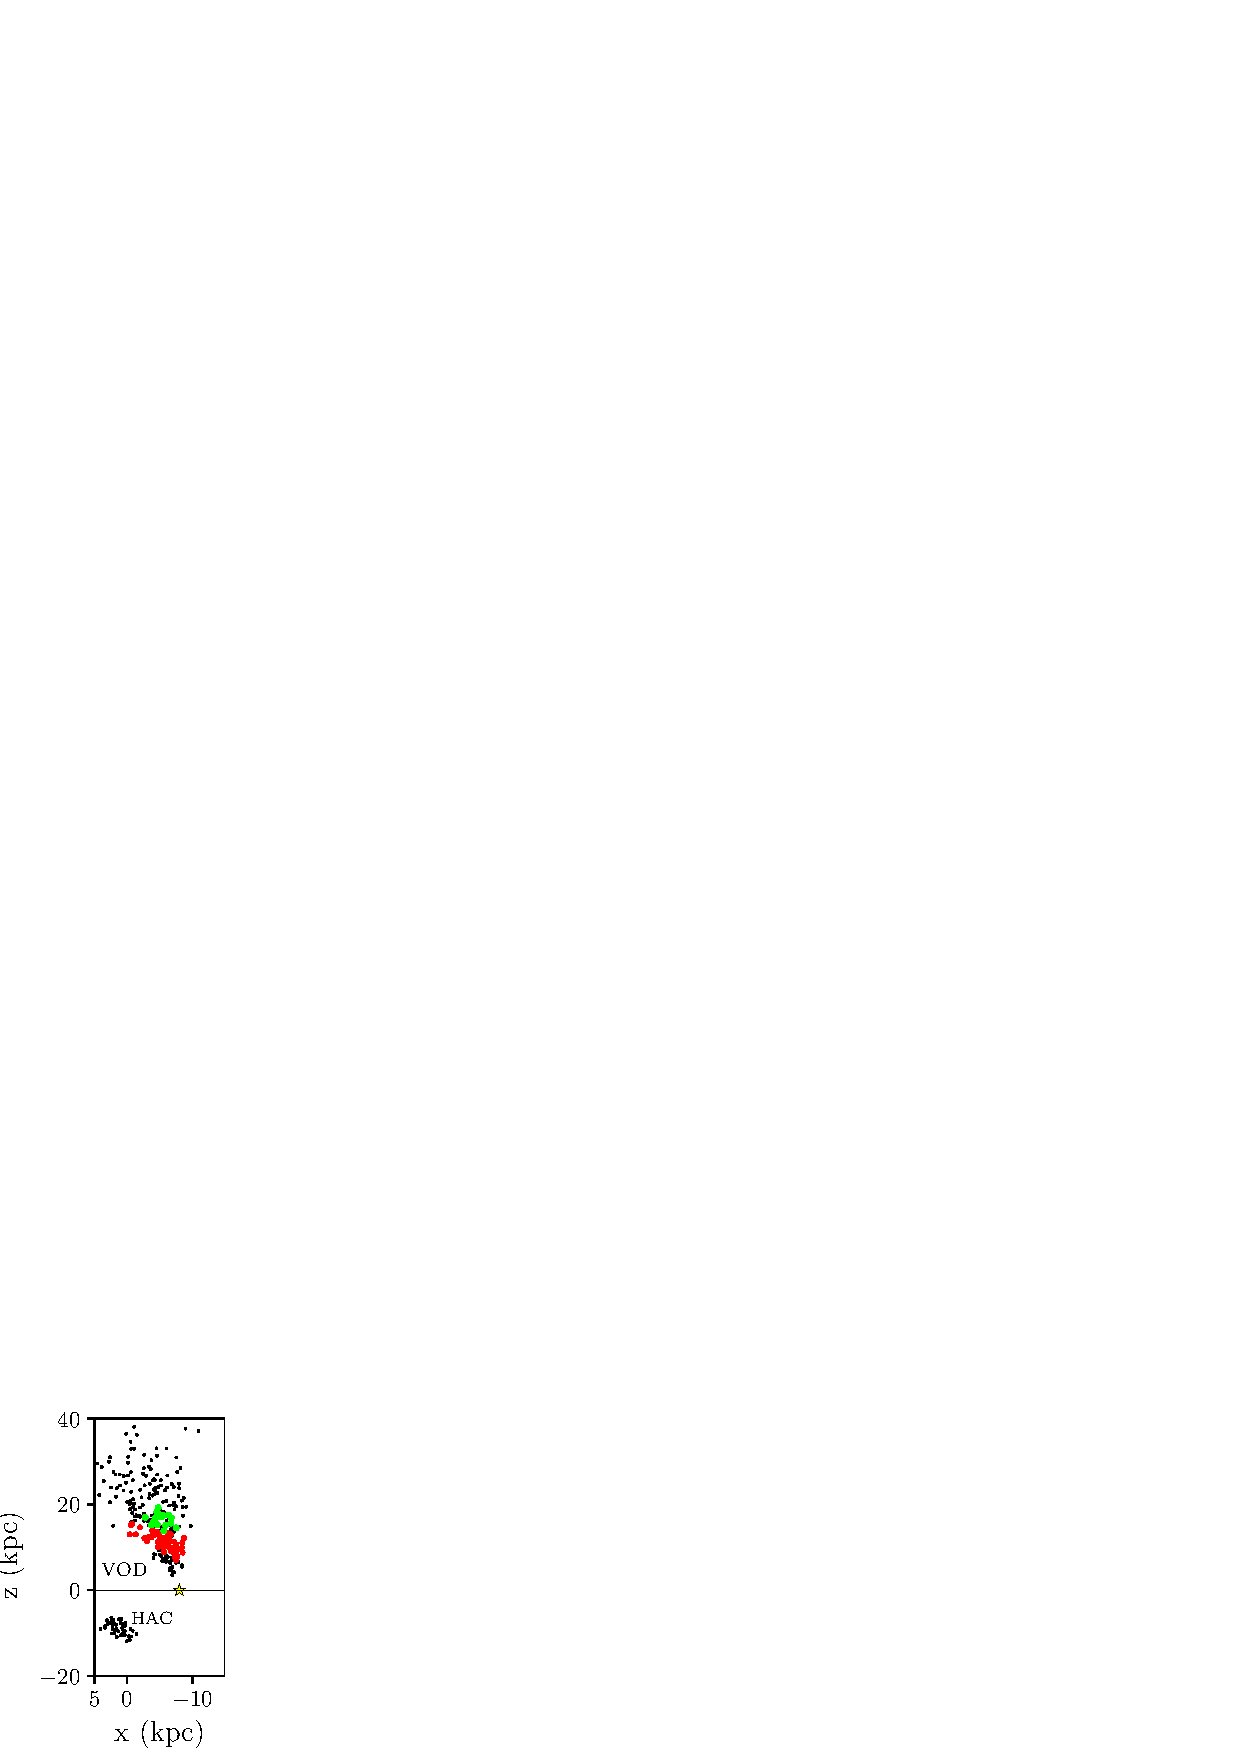
\includegraphics[scale=0.58]{xz.pdf}

    \caption{Spatial distribution of the RR Lyrae used in this work with full 6-D phase space measurements, in Galactic coordinates (left panel) and in the $x-y$ (middle) and $y-z$ (right) planes.  The HAC field contains 44 RR Lyrae which likely belong to the Cloud with measured line-of-sight  velocities (Simion et al. 2018) and  Gaia DR2 proper motions. The VOD field contains 411 RRL which belong to several halo associations, including the Sagittarius stream and the VOD, with line-of-sight velocities provided by Vivas et al. 2016 and proper motions from Gaia DR2. In particular we mark three `high significance' groups, excluding the Sagittarius stream,  identified by Vivas et al. 2016: `group 2' contains 18 stars (green circles), `group 3', 7 stars (orange squares) and `group 4', 5 stars (blue triangles). Two other `high significance' groups are not marked in this figure as they are situated at distances larger than 30 kpc and contain only 3 stars each. We exclude from all the plots in this letter `group 1' which contains Sagittarius members (112 stars). The Sun (yellow star) is located at (x$_{\odot}$, y$_{\odot}$, z$_{\odot})= $ (0,-8,0) kpc .  }
    \label{fig:lb}
\end{figure*}

% Example figure
\begin{figure}
	% To include a figure from a file named example.*
	% Allowable file formats are eps or ps if compiling using latex
	% or pdf, png, jpg if compiling using pdflatex
	\includegraphics[scale=0.545]{HAC_velocities_vphi.pdf}
    \includegraphics[scale=0.545]{HAC_velocities_vtheta.pdf} \\
  \includegraphics[scale=0.545]{VOD_velocities_vphi.pdf}
    \includegraphics[scale=0.545]{VOD_velocities_vtheta.pdf}   \\
      \includegraphics[scale=0.545]{VOD_velocities_vphi_gm.pdf}
    \includegraphics[scale=0.545]{VOD_velocities_vtheta_gm.pdf} \\

    \caption{RRL velocity distribution in spherical polar coordinates ($v_{r}$, $v_{\theta}$, $v_{\phi}$  are the radial, azimuthal and polar components respectively) in the HAC field (top row) and the VOD field (middle and bottom rows). The error on the velocity components of each star $i $, [$\sigma^{i}_{v_{r}}$, $\sigma^{i}_{v_{\theta}}$, $\sigma^{i}_{v_{\phi}}$], has been propagated by randomly drawing 1000 stars from a multivariate Gaussian distribution with mean the measurement (ra$^{i}$, dec$^{i}$, d$^{i}$, pmra$^{i}$, pmdec$^{i}$, $v^{i}_{h}$) and full covariance matrix (takes into account the covariances between ra,dec and proper motions). The orbital anisotropy, is highly radial in the HAC field ($\beta = 0.88$) where the stars are most likely members of the Cloud and mildly radial in the VOD field ($\beta = 0.48$) in which stars span a much wider range of distances (see Fig. \ref{fig:lb}). We fit the VOD velocity ellipsoid with a two component Gaussian mixture model and the result is shown in the bottom row. Stars are colour coded by their probability to belong to each component. (NOTE: this is NOT extreme deconvolution -simply used sklearn.mixture.GaussianMixture with no contraints on any parameter-, no errors taken into account. Please have a look at the last figure for extreme deconvolution). }
    \label{fig:vel}
\end{figure}


\begin{figure}
	% To include a figure from a file named example.*
	% Allowable file formats are eps or ps if compiling using latex
	% or pdf, png, jpg if compiling using pdflatex
	        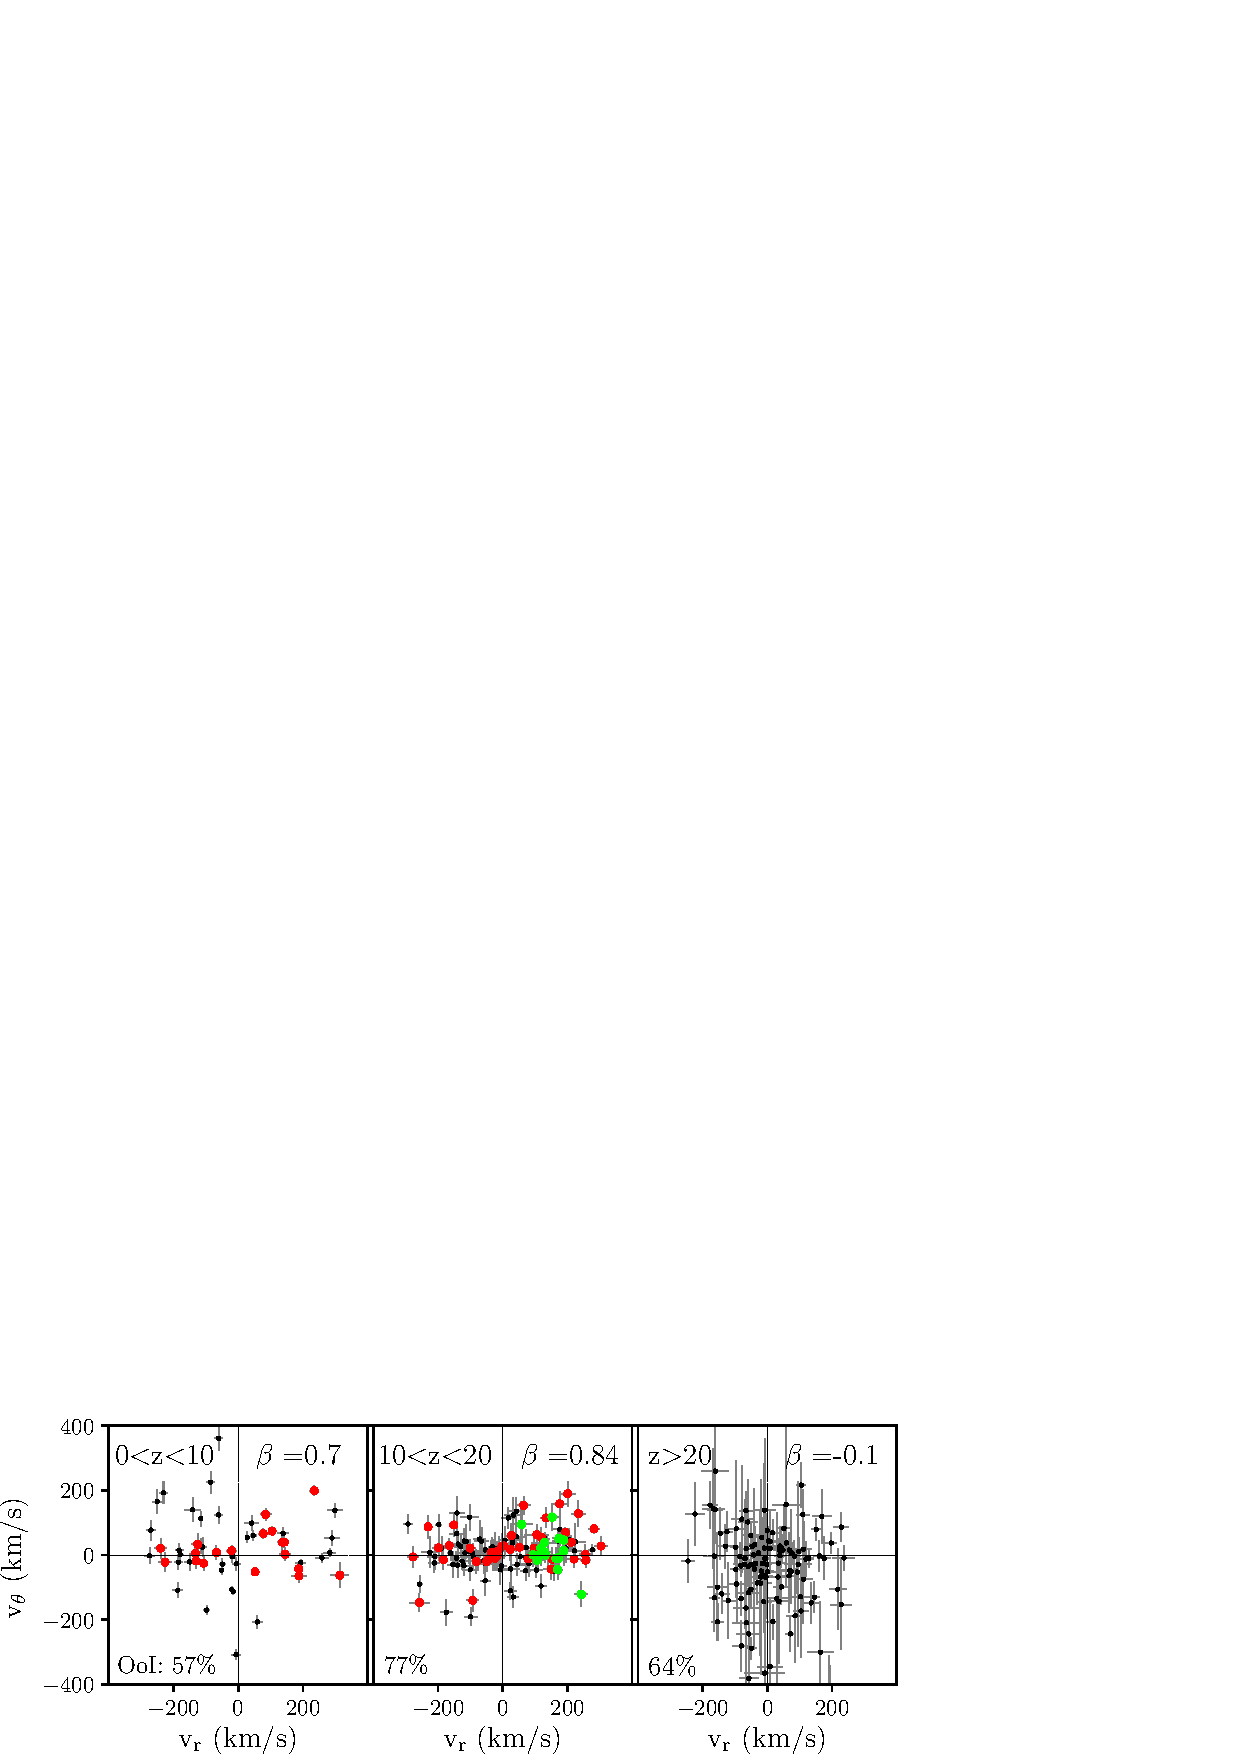
\includegraphics[scale=0.555]{VOD_velocities_vphi_zcuts.pdf}
   \caption{Radial versus azimuthal velocity in the VOD field, in three slices of Z, colour coded as in the bottom row of Fig. \ref{fig:vel}. We calculate the fraction of RR Lyrae of Oosterhoff type I and II (reported in each panel for Oo I) and find that in the 10$<$z/kpc$<$20 range, where the orbital anisotropy is the highest, the Oo I type dominates  (77\%), as in the HAC field (note: add number here). In the same slice, 73\% of the stars belong to the `sausage' component. The same behaviour but less accentuated can be noticed in the 0$<$z/kpc$<$10 slice where $\beta$ is  less radial but the fraction of Oo I stars decreases drammatically (note: comment if this is expected?). Further from the plane, at  z$>$20 kpc, the velocity ellipsoid is almost isotropic with $\beta = -0.3$. We have excluded the most likely members of the Sagittarius stream but several others may remain, decreasing $\beta$.  (note: I should add constant z lines in the right panel of figure 1 if we keep this). This figure should replace the bottom row of Figure 2? - }
    \label{fig:VOD_vel}
\end{figure}

\begin{figure}
	% To include a figure from a file named example.*
	% Allowable file formats are eps or ps if compiling using latex
	% or pdf, png, jpg if compiling using pdflatex
	\includegraphics[scale=0.472]{HAC_orbits_ecc_z.pdf}
    \includegraphics[scale=0.472]{HAC_orbits_apo_ecc.pdf} 
  \includegraphics[scale=0.472]{HAC_orbits_ecc_r.pdf} \\
	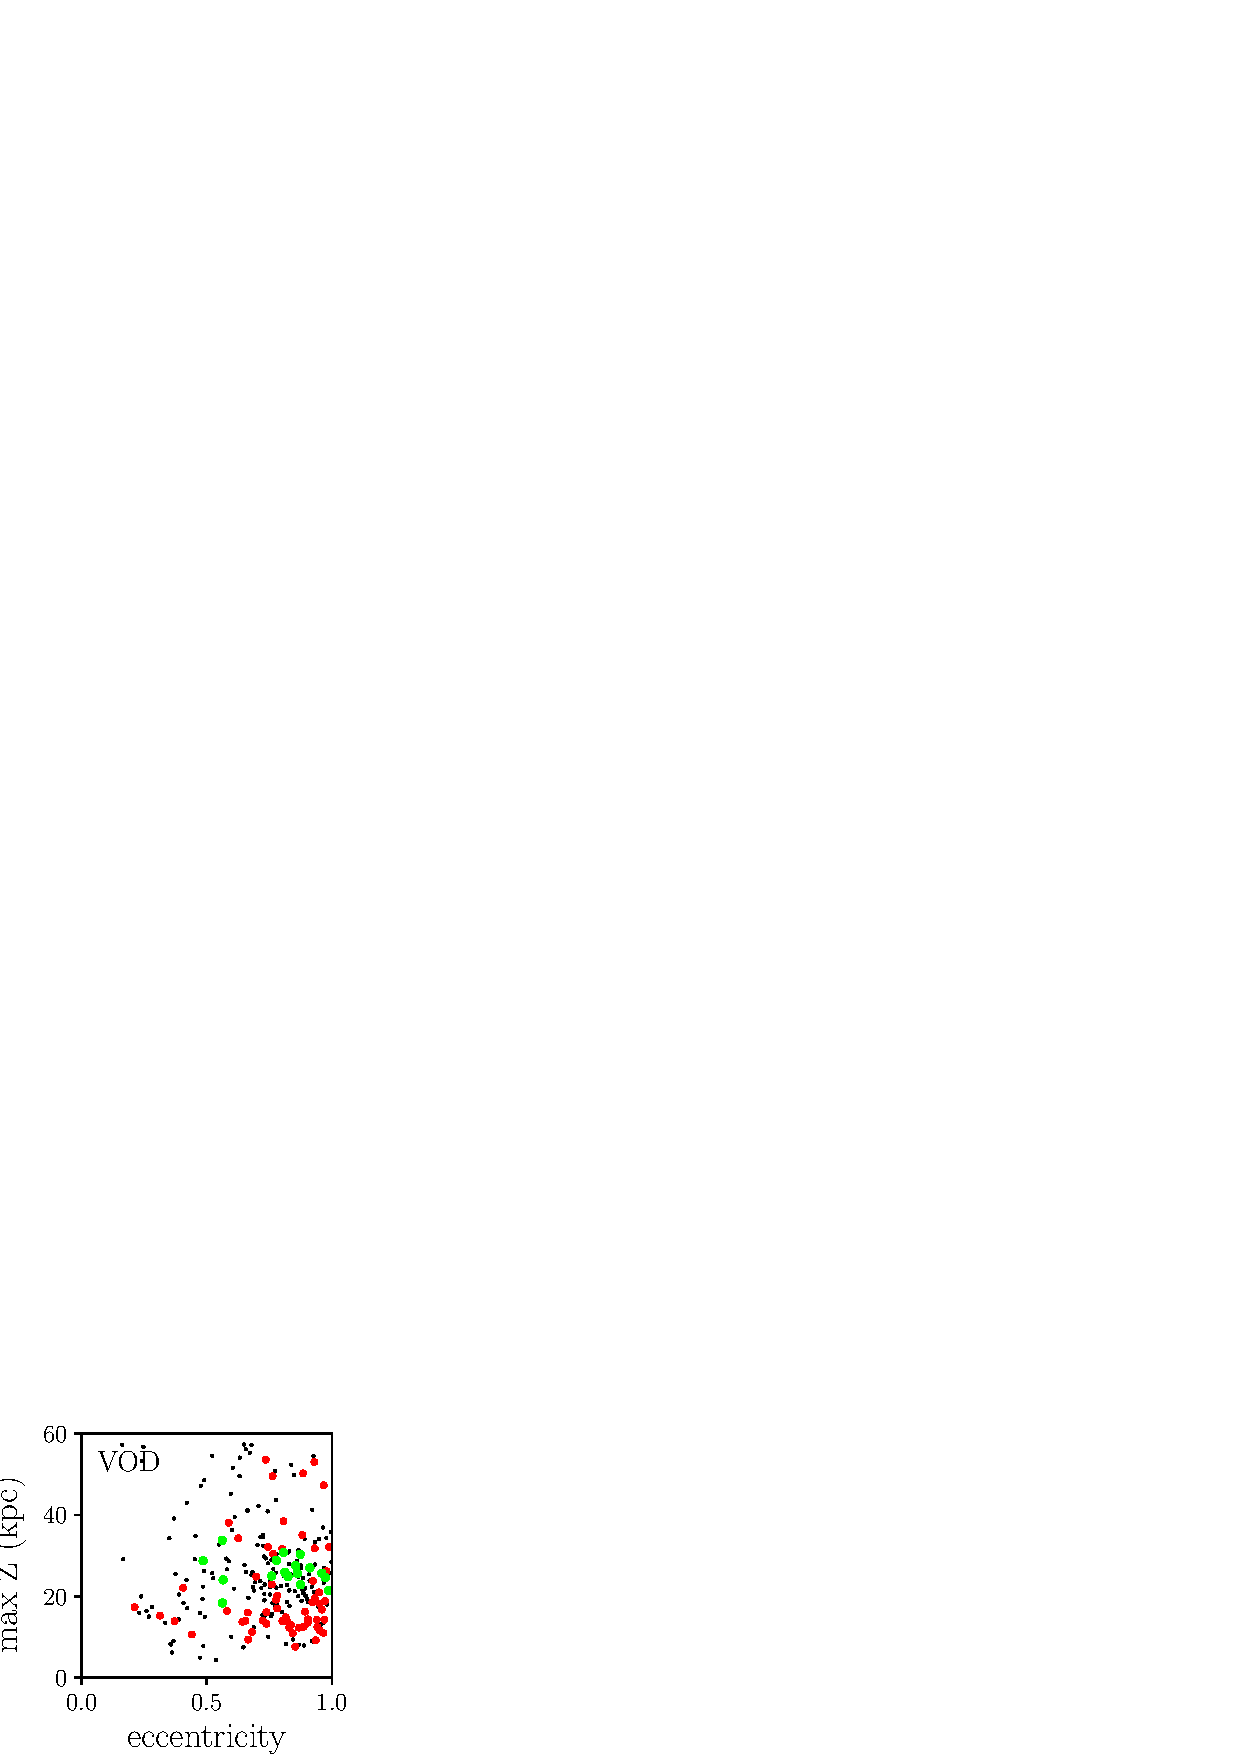
\includegraphics[scale=0.472]{VOD_orbits_ecc_z.pdf}
    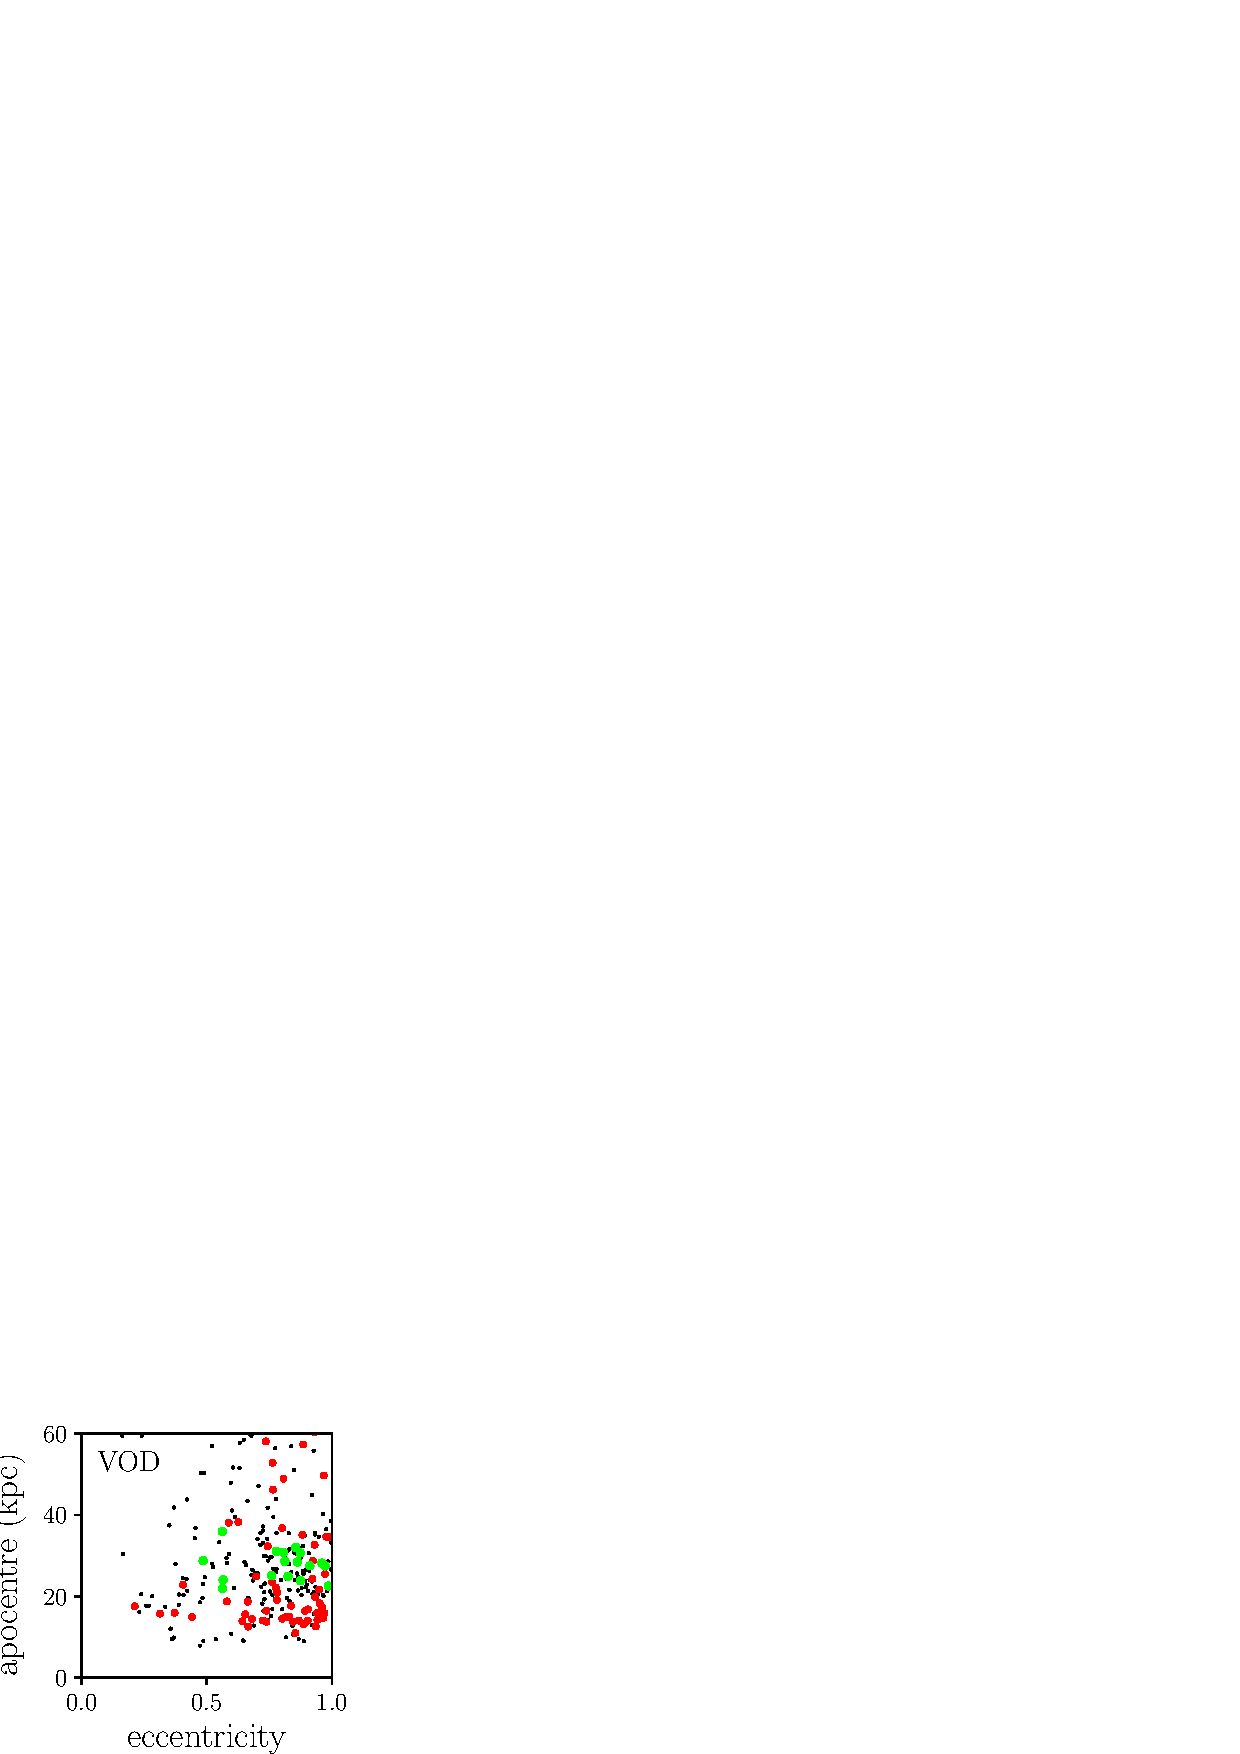
\includegraphics[scale=0.472]{VOD_orbits_apo_ecc.pdf} 
  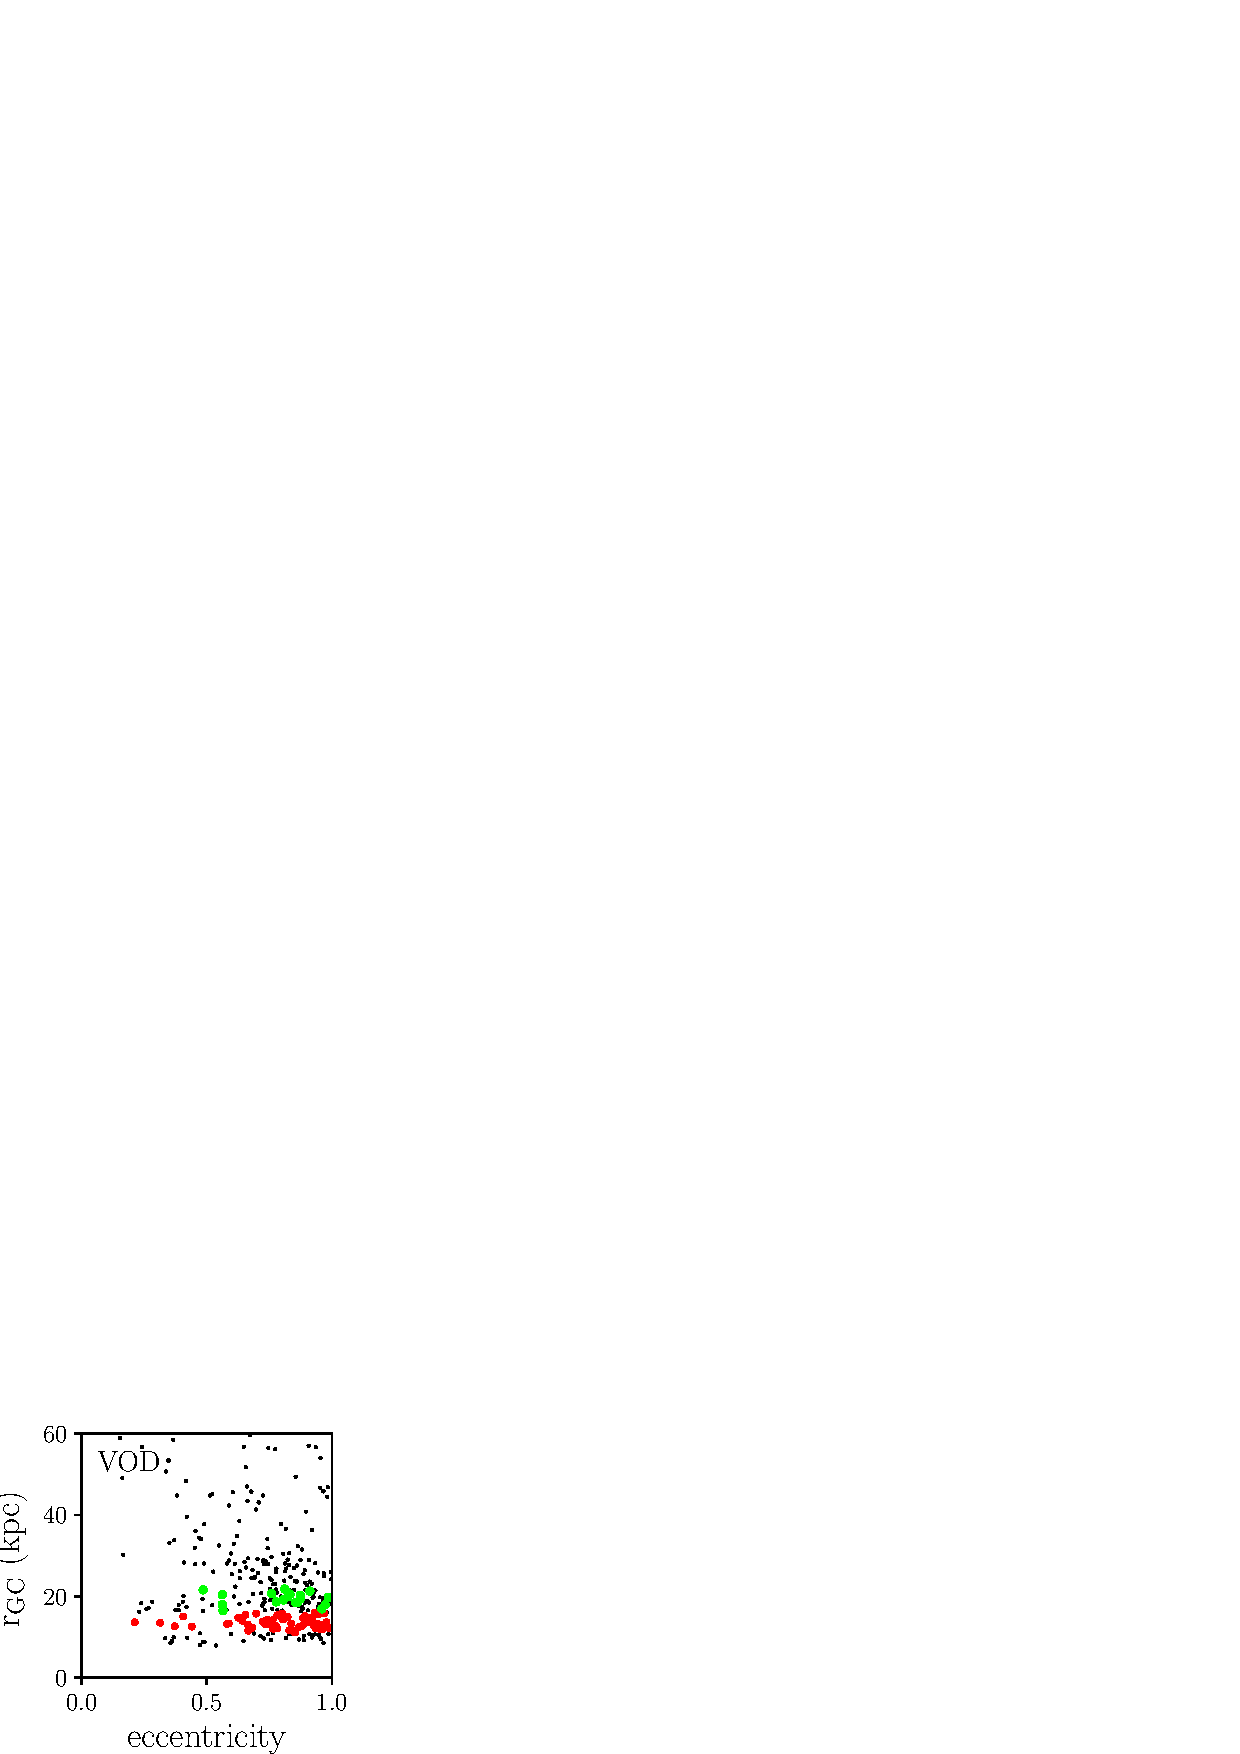
\includegraphics[scale=0.472]{VOD_orbits_ecc_r.pdf} 
    \caption{ Orbital properties of the stars in the HAC and VOD fields. `group 2' has similar orbital properties to the HAC, however it does not display a sausage velocity distribution (see middle row figure 2) - they are concentrated at $vr =  135 $km/s as calculated by Vivas et al. 2016. }
    \label{fig:orbits}
\end{figure}


\begin{figure}
	% To include a figure from a file named example.*
	% Allowable file formats are eps or ps if compiling using latex
	% or pdf, png, jpg if compiling using pdflatex
    \includegraphics[scale=0.472]{VOD_velocities_vphi_z0_10_bytype.pdf}  
	\includegraphics[scale=0.472]{VOD_velocities_vphi_z10_20_bytype.pdf}
    \includegraphics[scale=0.472]{VOD_velocities_vphi_z20_60_bytype.pdf} \\
\includegraphics[scale=0.472]{VOD_velocities_vphi_zcol.pdf}
   \caption{EXTRA: top row: only these stars pass the RR ab cuts (equation 1 in your RR Lyrae paper). In pink I mark the Oo II type. The fractions I reported in Figure 3, are based on these figures. bottom row: this is Figure 3, just colour coded by z instead of showing 3 different cuts. I liked the cuts because it's very easy to see the anisotropy is the highest in the 10$<z<$20 range, like the HAC. }
    \label{fig:example_figure}
\end{figure}



\begin{figure}
	% To include a figure from a file named example.*
	% Allowable file formats are eps or ps if compiling using latex
	% or pdf, png, jpg if compiling using pdflatex
	       \includegraphics[scale=0.545]{VOD_velocities_vphi_gm2.pdf}
    \includegraphics[scale=0.545]{VOD_velocities_vtheta_gm2.pdf} \\
   \includegraphics[scale=0.545]{VOD_velocities_vphi_gm3.pdf}
    \includegraphics[scale=0.545]{VOD_velocities_vtheta_gm3.pdf} \\

   \caption{EXTRA: Extreme deconvolution with 2 (top) and 3 (bottom) components. Should I add some constraints on the parameters? I also tried to fit by z slices and I find the same behaviour. }
    \label{fig:xd}
\end{figure}
\section{Conclusions}

The last numbered section should briefly summarise what has been done, and describe
the final conclusions which the authors draw from their work.

\section*{Acknowledgements}

The Acknowledgements section is not numbered. Here you can thank helpful
colleagues, acknowledge funding agencies, telescopes and facilities used etc.
Try to keep it short.

%%%%%%%%%%%%%%%%%%%%%%%%%%%%%%%%%%%%%%%%%%%%%%%%%%

%%%%%%%%%%%%%%%%%%%% REFERENCES %%%%%%%%%%%%%%%%%%

% The best way to enter references is to use BibTeX:

%\bibliographystyle{mnras}
%\bibliography{example} % if your bibtex file is called example.bib


% Alternatively you could enter them by hand, like this:
% This method is tedious and prone to error if you have lots of references
\begin{thebibliography}{99}
\bibitem[\protect\citeauthoryear{Author}{2012}]{Author2012}
Author A.~N., 2013, Journal of Improbable Astronomy, 1, 1
\bibitem[\protect\citeauthoryear{Others}{2013}]{Others2013}
Others S., 2012, Journal of Interesting Stuff, 17, 198
\end{thebibliography}

%%%%%%%%%%%%%%%%%%%%%%%%%%%%%%%%%%%%%%%%%%%%%%%%%%

%%%%%%%%%%%%%%%%% APPENDICES %%%%%%%%%%%%%%%%%%%%%

\appendix

\section{Some extra material}

If you want to present additional material which would interrupt the flow of the main paper,
it can be placed in an Appendix which appears after the list of references.

%%%%%%%%%%%%%%%%%%%%%%%%%%%%%%%%%%%%%%%%%%%%%%%%%%


% Don't change these lines
\bsp	% typesetting comment
\label{lastpage}
\end{document}

% End of mnras_template.tex